\section{Projekt \textit{auctioneer}}

Poniżej zaprezentowano rezultat pracy nad projektem \textit{auctioneer}.

\subsection{Architektura}

Aplikacje pisane przy użyciu aplikacji szkieletowej Ruby~on~Rails opierają się na~architekturze \textit{MVC} (ang.~\textit{model-view-controller}). Oznacza to, że~w~aplikacji takiej wyróżnione są~warstwy odpowiedzialne za~dostęp do~danych i~ich ,,obróbkę'', realizację logiki biznesowej aplikacji oraz prezentację (interfejs graficzny).

\subsubsection{Warstwa danych -- model}

Ruby~on~Rails wykorzystuje moduł \texttt{ActiveRecord} do~opakowania rekordów, pochodzących z~relacyjnych baz danych, odpowiadającymi im obiektami. Dzięki temu programista może traktować tabele bazy danych jako klasę, a~rekordy tej tabeli jako jej instancje.

\begin{itemize}
  \item[admins]\hfill\\ reprezentacja danych modelu administratora; zawiera adres e-mail, zaszyfrowane hasło, stemple czasu (utworzenie i edycja rekordu) oraz dane logowania (stempel czasu, adres IP, z~którego się zalogowano),
  \item[users]\hfill\\ reprezentacja danych modelu użytkownika; zwiera adres e-mail, zaszyfrowane hasło, stemple czasu, dane logowania oraz dane aktywacji konta,
  \item[auctions]\hfill\\ reprezentacja danych modelu aukcji; zawiera tytuł, opis, cenę minimalną i~aktualną aukcji, aktualny stan, klucze (identyfikatory) użytkownika-właściciela i~użytkownika-zwycięzcy oraz stemple czasu.
\end{itemize}

Na~rysunku \ref{database} zamieszczono schemat tabeli bazy danych projektu \textit{auctioneer}. Listingi \ref{code.auction}, \ref{code.admin}, \ref{code.user} pokazują klasy opakowujące dane dla modeli projektu \textit{auctioneer}.

\begin{figure}[h]
\centering
\fbox{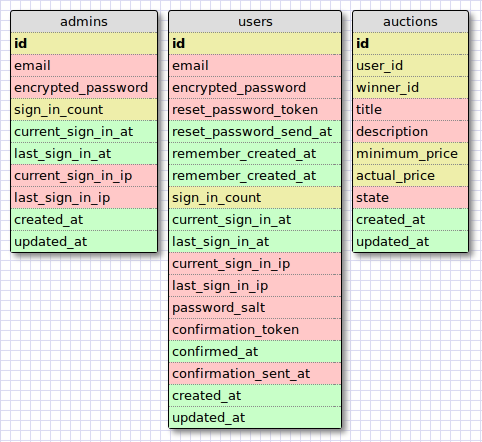
\includegraphics[width=0.6\textwidth]{obrazki/entity.png}}
\caption{Schemat bazy danych projektu \textit{auctioneer}}
\label{database}
\end{figure}

\lstset{language=Ruby, caption=Klasa reprezentacji modelu aukcji, basicstyle=\ttfamily\footnotesize, numbers=left, numberstyle=\footnotesize, captionpos=b, backgroundcolor=\color{LightGray}}
\begin{lstlisting}[label={code.auction}]
class Auction < ActiveRecord::Base
  EXPIRATION_AFTER = 7.days

  belongs_to :user
  belongs_to :winner, class_name: 'User'
  validates :title, presence: true
  validates :minimum_price, presence: true

  scope :created, where(state: :new)
  scope :public, where(state: :public)
  scope :closed, where(state: :closed)
  scope :won, where(state: :won)
  scope :finished, where('state = "closed" OR state = "won"')
  scope :won_by, ->(user) { where(state: :won).where(winner_id: user.id) }

  def self.about_to_finish
    time = Time.now
    now = Time.new(time.year, time.month, time.day, time.hour, 0)
    where(state: :public).
    where('created_at < ?', now - EXPIRATION_AFTER + 1.hour).
    where('created_at >= ?', now - EXPIRATION_AFTER)
  end

  # scope used in search engine
  def self.search(query)
    if query
      phrase = "%#{query}%"
      where('(title LIKE ?) OR (description LIKE ?)', phrase, phrase)
    else
      scoped
    end
  end

  # closing every expired auction
  def self.close_auctions
    self.about_to_finish.each do |auction|
      auction.close if auction.winner.nil?
      auction.win if auction.winner.present?
    end
  end

  state_machine initial: :new do
    after_transition any => :public do |auction, transition|
      auction.actual_price = auction.minimum_price
      auction.save!
    end

    event :publish do
      transition new: :public, if: ->(auction) {
        auction.description.present?
      }
    end

    event :close do
      transition public: :closed
    end

    event :win do
      transition public: :won, if: ->(auction) {
        auction.actual_price != auction.minimum_price && auction.winner.present?
      }
    end

    event :republish do
      transition closed: :public
    end
  end

end
\end{lstlisting}

\lstset{language=Ruby, caption=Klasa reprezentacji modelu administratora, basicstyle=\ttfamily\footnotesize, numbers=left, numberstyle=\footnotesize, captionpos=b, backgroundcolor=\color{LightGray}}
\begin{lstlisting}[label={code.admin}]
class Admin < ActiveRecord::Base
  devise :database_authenticatable, :trackable, :validatable,
         :timeoutable
  attr_accessible :email, :password, :password_confirmation
  validates_presence_of :email
  validates_uniqueness_of :email, case_sensitive: false

  scope :email_like, ->(email) { where('admins.email like ?', email) }
end
\end{lstlisting}

\lstset{language=Ruby, caption=Klasa reprezentacji modelu użytkownika, basicstyle=\ttfamily\footnotesize, numbers=left, numberstyle=\footnotesize, captionpos=b, backgroundcolor=\color{LightGray}}
\begin{lstlisting}[label={code.user}]
class User < ActiveRecord::Base
  devise :database_authenticatable, :registerable, :recoverable,
         :rememberable, :trackable, :validatable, :confirmable
  attr_accessible :email, :password, :password_confirmation,
         :remember_me
  validates_presence_of :email
  validates_uniqueness_of :email, case_sensitive: false
  has_many :auctions

  scope :email_like, ->(email) { where('users.email like ?', email) }
end
\end{lstlisting}

\subsubsection{Warstwa logiki -- kontroler}

\textit{Kontroler} jest elementem decyzyjnym realizującym założenia logiki biznesowej projektu. W~Ruby~on~Rails kontrolerami są~pewne klasy, które grupują w~sobie metody (tak zwane akcje). Akcje są~wykonywane podczas każdego zapytania HTTP. O~tym, która akcja zostanie wykonana, decyduje system rozpoznawania ścieżek i~parametrów zapytania -- \texttt{routes}. Listing \ref{code.controller} prezentuje przykładowy kontroler dla aplikacji \textit{auctioneer}.

\lstset{language=Ruby, caption=Przykładowy kontroler \texttt{Admin::UsersController} odpowiadający za~akcje związane z~zarządzaniem użytkownikami w panelu administratora, basicstyle=\ttfamily\footnotesize, numbers=left, numberstyle=\footnotesize, captionpos=b, backgroundcolor=\color{LightGray}}
\begin{lstlisting}[label={code.controller}]
class Admin::UsersController < ApplicationController
  before_filter :authenticate_admin!
  layout 'admin'

  def index
    @users = User.email_like(params[:like] || '%').paginate(page: params[:page])
  end

  def destroy
    @user = User.find(params[:id]).destroy
    flash[:notice] = t('admin.registrations.destroy')
    redirect_to admin_users_path
  end

  def login
    sign_in(:user, User.find(params[:id]))
    redirect_to root_path
  end

  def confirm
    User.find(params[:id]).confirm!
    redirect_to admin_users_path
  end
end
\end{lstlisting}

\subsubsection{Warstwa prezentacji -- widok}

Widoki to~szablony, generujące rezultaty -- odpowiedzi na~zadane zapytania protokołu HTTP. Są one wynikiem działania akcji kontrolera. W~aplikacji \textit{auctioneer} użyto metajęzyka \texttt{haml} do~tworzenia takich szablonów. Listing \ref{code.view} przedstawia przykładowy szablon widoku.

\lstset{language=Ruby, caption=Przykładowy widok -- lista użytkowników w~panelu administratora, basicstyle=\ttfamily\footnotesize, numbers=left, numberstyle=\footnotesize, captionpos=b, backgroundcolor=\color{LightGray}}
\begin{lstlisting}[label={code.view}]
= form_tag admin_users_path, method: :get do
  = label_tag :email, "Filter by email:"
  = text_field_tag :like, h(params[:email])
  = submit_tag "Filter"
  .grey
    use '%' to match anything (like '%examp%')

- unless params[:like].nil?
  %p
    Filtered with
    %strong
      = h(params[:like])

= will_paginate(@users)

%table
  %tr
    %th Email
    %th Created at
    %th Confirmed at
    %th Last signed in
    %th Sign in IP
    %th{ colspan: 2 } Actions
  - @users.each do |user|
    %tr
      %td= user.email
      %td= user.created_at
      %td= user.confirmed_at.present? ? user.confirmed_at : 'not confirmed yet'
      %td= user.last_sign_in_at.present? ? user.last_sign_in_at : 'not signed in yet'
      %td= user.last_sign_in_at.present? ? user.last_sign_in_ip : 'not signed in yet'

      - if user.confirmed?
        %td= link_to 'Sign in', admin_user_login_path(user)
      - else
        %td= link_to 'Confirm', admin_user_confirm_path(user)
      %td= link_to 'Delete', admin_user_delete_path(user), confirm: 'Are you sure?'

= will_paginate(@users)
\end{lstlisting}

\subsection{Testy}

W~realizacji poszczególnych funkcjonalności systemu ważną rolę spełniają testy. Stanowią one potwierdzenie poprawnego działania poszczególnych komponentów, a także chronią programistę przed popełnieniem nie przewidzianego błędu.

\subsubsection{Testy jednostkowe}

Testy jednostkowe \texttt{rspec} sprawdzają poprawność działania elementów logiki biznesowej, metod pomocniczych dla warstwy danych i~widoku oraz reakcji na zapytania HTTP. Testy jednostkowe znajdują się w~katalogu \texttt{spec}. Po~wywołaniu komendy \verb+rake spec+ aplikacja zostaje przetestowana. Wyniki takiego testowania zawiera listing \ref{code.spec}.

\lstset{language=Ruby, caption=Wyniki testowania aplikacji narzędziem \texttt{rspec}, basicstyle=\ttfamily\footnotesize, numbers=left, numberstyle=\footnotesize, captionpos=b, backgroundcolor=\color{LightGray}}
\begin{lstlisting}[label={code.spec}]
$ rake spec
ApplicationController
  routing
    routes to static_admin/admins#dashboard
    routes to static_admin/admins#index
    routes to static_admin/users#index
    routes to static_static_pages#landing

AuctionsController
  routing
    routes to #index
    routes to #show
    routes to #new
    routes to #edit
    routes to #create
    routes to #update
    routes to #destroy

Auction
  about_to_finish
    should not be empty
  about_to_finish
    should be empty
  about_to_finish
    should be empty
  close_auctions
    should eq 1

AdminHelper
  total_count_of
    should return a quantity of all records in model

AuctionsHelper
  short_description
    should return a shorten text with no html tags and ended with '...'

ApplicationHelper
  after_sign_in_path_for
    should return a proper url

Finished in 6.98 seconds
18 examples, 0 failures
\end{lstlisting}

\subsubsection{Testy behawioralne}

Testy behawioralne sprawdzają zachowanie aplikacji przy zadanych warunkach. W~projektach Ruby~on~Rails zwykle używa się w~tym celu narzędzia \textit{cucumber}. Testy takie składają się z~tak zwanych scenariuszy. Scenariusz to~lista kroków, w~których realizowane są poszczególne działania w~aplikacji oraz sprawdzane założenia. Testy behawioralne wraz z~konfiguracją środowiska testującego znajdują się w~katalogu \texttt{features}. Po~wywołaniu komendy \verb+rake cucumber+ aplikacja zostaje przetestowana. Wyniki takiego testowania zawiera listing \ref{code.cukes}.

\lstset{language=Ruby, caption=Przykładowy scenariusz opisujący system rejestracji i~logowania użytkowników, basicstyle=\ttfamily\footnotesize, numbers=left, numberstyle=\footnotesize, captionpos=b, backgroundcolor=\color{LightGray}}
\begin{lstlisting}[label={code.cukes}]
Feature: User accounts
  In order to have a private account
  A user
  Wants to manage it

  Scenario: Registering a user account
    Given I am on the home page
    And no emails have been sent
    When I follow "Sign up"
    And I fill in the following:
      | user_email                 | user@example.com |
      | user_password              | monkey           |
      | user_password_confirmation | monkey           |
    And I press "Sign up"
    Then "user@example.com" should receive an email
    When "user@example.com" opens the email
    Then I should see "Confirmation instructions" in the email subject
    And I should see "You can confirm your account" in the email body
    And I should see "Confirm my account" in the email body
    When I follow "Confirm my account" in the email
    And I should see "Sign out"

  Scenario: Changing users password
    Given a user "quentin"
    And I am on the home page
    When I follow "Sign in"
    And I follow "Forgot your password?"
    And I fill in the following:
      | user_email | quentin@example.com |
    And I press "Send me reset password instructions"
    Then I should see "You will receive an email with instructions"
    And "quentin@example.com" should receive an email
    When "quentin@example.com" opens the email
    Then I should see "Reset password instructions" in the email subject
    And I should see "link to change your password" in the email body
    When I follow "Change my password" in the email
    Then I should see "Change your password"
    When I fill in the following:
      | user_password              | monkey |
      | user_password_confirmation | monkey |
    And I press "Change my password"

  Scenario: Resend a confirmation instructions
    Given I am on the home page
    And an unconfirmed user "user"
    And a clear email queue
    When I follow "Sign up"
    And I follow "Didn't receive confirmation instructions?"
    Then I should see "Resend confirmation instructions"
    When I fill in the following:
      | user_email | user@example.com |
    And I press "Resend confirmation instructions"
    Then I should see "You will receive an email with instructions"
    And "user@example.com" should receive an email
    When "user@example.com" opens the email
    Then I should see "Confirmation instructions" in the email subject
    And I should see "You can confirm your account" in the email body

  Scenario: Logging in and out
    Given a user "quentin"
    And I am on the home page
    When I follow "Sign in"
    And I fill in the following:
      | user_email    | quentin@example.com |
      | user_password | secret              |
   And I press "Sign in"
   Then I should see "quentin@example.com"
\end{lstlisting}

\subsection{Dziennik realizacji zadań}

Realizacja poszczególnych zadań ma~swoje odzwierciedlenie w~historii kodu w~repozytorium \textit{Git}. Poniżej przedstawiono historię zmian kodu.

\begin{verbatim}
* 5f69148: changes in report; closed chapter describing application
* 1b8d6b1: changes in report; minor changes in application
* cf54641: removed ruby-debug from Gemfile
* 8c2da87: another changes due to report
* 99ba8ff: added new content to report; some small corrections
* d360dfa: fixed spec tests for auction model
* fd1c522: changes in report; added new chapter
* a2fb439: [#134409] added simple relancing system with hourly checking for winners
* 9eb16d9: [#8269df] ordering the search results by title, minimum and actual price
* 4707b6a: some more resolution to report
* f73219b: changes in report due to suggestions
* 9bd648b: [#378254] simple search engine added
* c5a3008: [#b2296e] auctions are treated as state machine
*   c9526a7: Merging branches
|\
| * 2c1e199: [#fca367 and #ed753d] simple schema of auctioning system
| * bcc6b5a: [#fca367] changes in admin and user models; prepared devise system
* | b234283: removed pdf file from documentation
* | 6ce2ac8: more specific documentation about used tools
* | 2972c55: some logical changes in report
* | 2017f51: added a doc directory containing a documentation
* | 8c8cb9a: [#fca367] added admin and user models;
|/
* 836ffa3: removed unnecesary README_FOR_APP file
* 17550e4: [#36ce13] added localization scopes
* f42d5dc: first commit; new project created; initialized gems
\end{verbatim}

\section{Podręcznik użytkownika}

Poniżej zamieszczono opis stworzonej aplikacji od~strony osoby jej użytkującej. Osobą taką może być jeden z~trzech aktorów: gość, zwykły użytkownik oraz administrator. Możliwe działania dla poszczególnych aktorów tworzą scenariusze dla poszczególnych przypadków użycia. Założono, że~punktem wyjścia jest odwiedzenie przez aktora strony głównej projektu (Rys. \ref{screen01}).

\begin{figure}[h]
\centering
\fbox{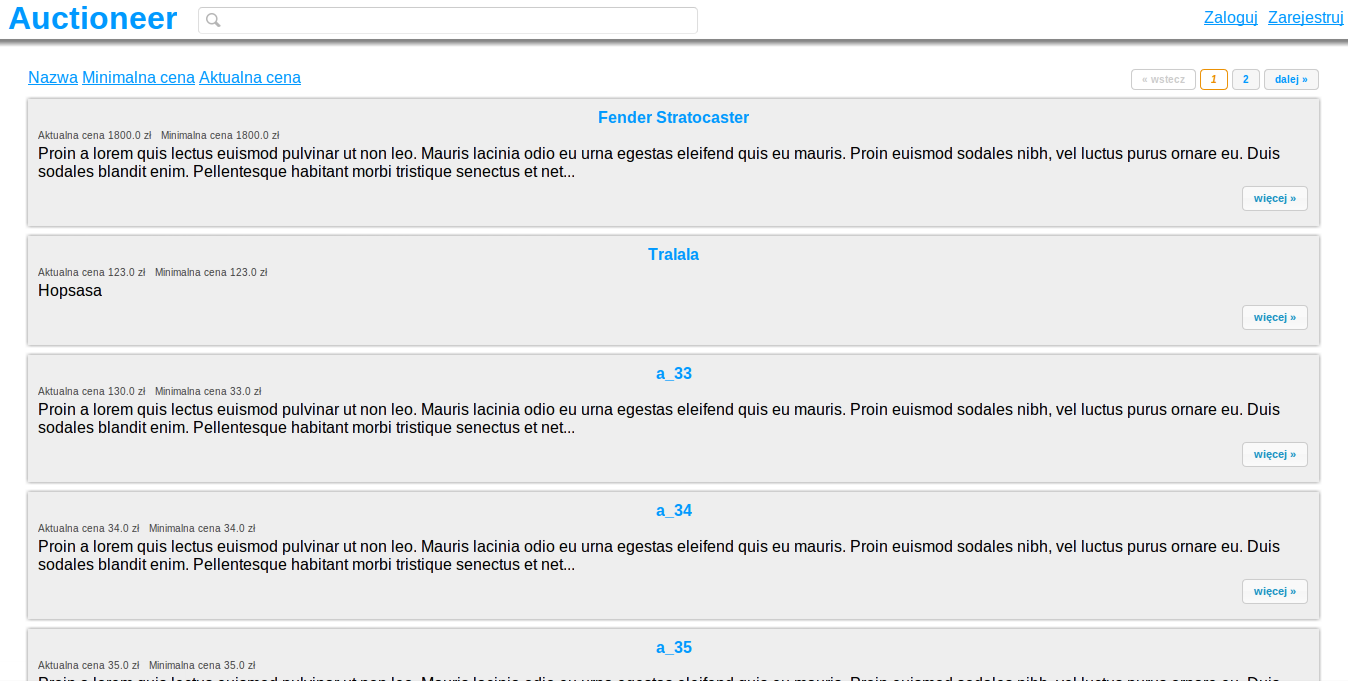
\includegraphics[width=\textwidth]{obrazki/auctioneer01.png}}
\caption{Strona główna serwisu \textit{auctioneer} -- lista wystawionych aukcji}
\label{screen01}
\end{figure}

\subsection{Opis projektu od strony gościa}

\paragraph{Strona główna}

Na~stronie głównej znajdują się następujące aktywne elementy:

\begin{itemize}
  \item pole tekstowe wyszukiwarki aukcji,
  \item link ,,Zaloguj'',
  \item link ,,Zarejestruj'',
  \item link ,,Nazwa'',
  \item link ,,Minimalna cena'',
  \item link ,,Aktualna cena'',
  \item zestaw przycisków: ,,wstecz'', ,,1'', ,,2'', \ldots, ,,dalej'',
  \item lista aukcji,
  \item link-nagłówek ,,Auctioneer''.
\end{itemize}

Pole tekstowe wyszukiwarki aukcji pozwala na~wyselekcjonowanie aukcji, znajdujących się w~liście poniżej, według zadanych kryteriów. Wpisanie wyszukiwanej frazy oraz~wciśnięcie klawisza \texttt{Enter} spowoduje przejście do~strony z~wynikami wyszukiwania (Rys. \ref{screen02}). Strona z~wynikami wyszukiwania jest podobna do~strony głównej, z~tą~różnicą, że~ponad wynikami wyszukiwania widoczna jest informacja na~temat wyszukiwanej frazy.

\begin{figure}[h]
\centering
\fbox{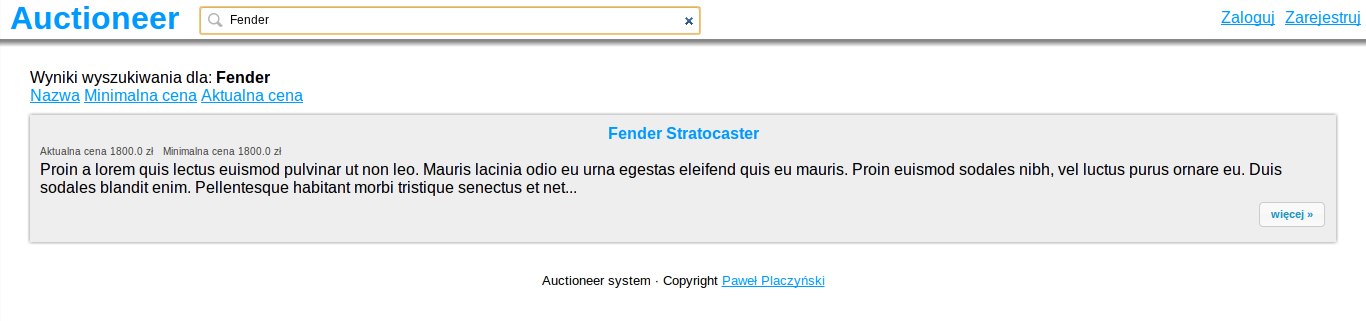
\includegraphics[width=\textwidth]{obrazki/auctioneer02.png}}
\caption{Działanie wyszukiwarki aukcji serwisu \textit{auctioneer}}
\label{screen02}
\end{figure}

Link ,,Zaloguj'' przekierowuje gościa do~formularza logowania (Rys. \ref{screen03}). Formularz logowania opisany został poniżej. Link ,,Zarejestruj'' przekierowuje do~formularza rejestracji (Rys. \ref{screen13}). Zestaw odsyłaczy: ,,Nazwa'', ,,Minimalna cena'' oraz ,,Aktualna cena''  zmienia kolejność wyświetlania aukcji, sortując je~według nazwy, minimalnej oraz aktualnej ceny (ponowne wybranie linku odwraca kolejność sortowania). Link-nagłówek ,,Auctioneer'' prowadzi zawsze na~stronę główną.

\begin{figure}[h]
\centering
\fbox{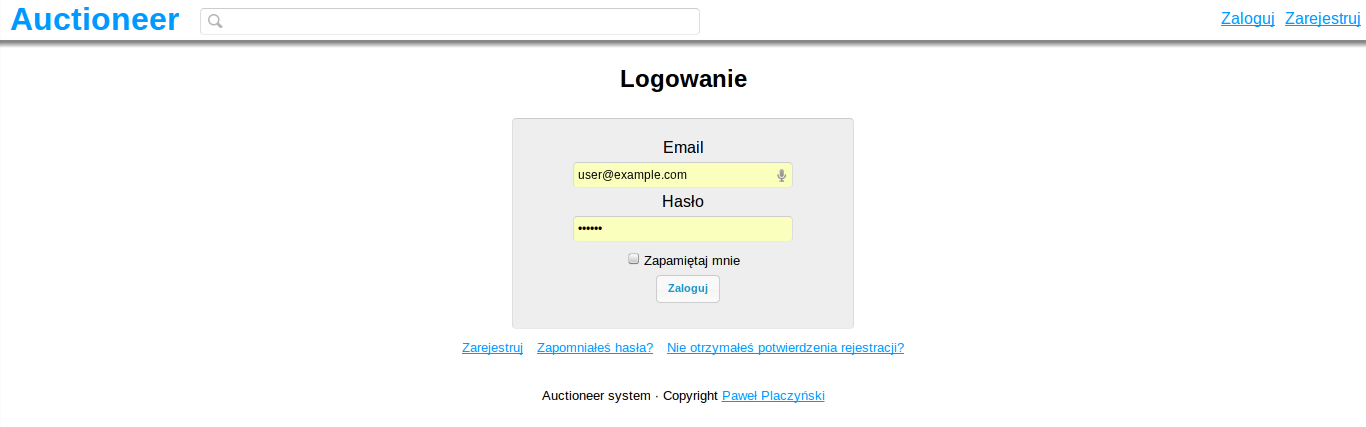
\includegraphics[width=\textwidth]{obrazki/auctioneer03.png}}
\caption{Ekran logowania}
\label{screen03}
\end{figure}

\begin{figure}[h]
\centering
\fbox{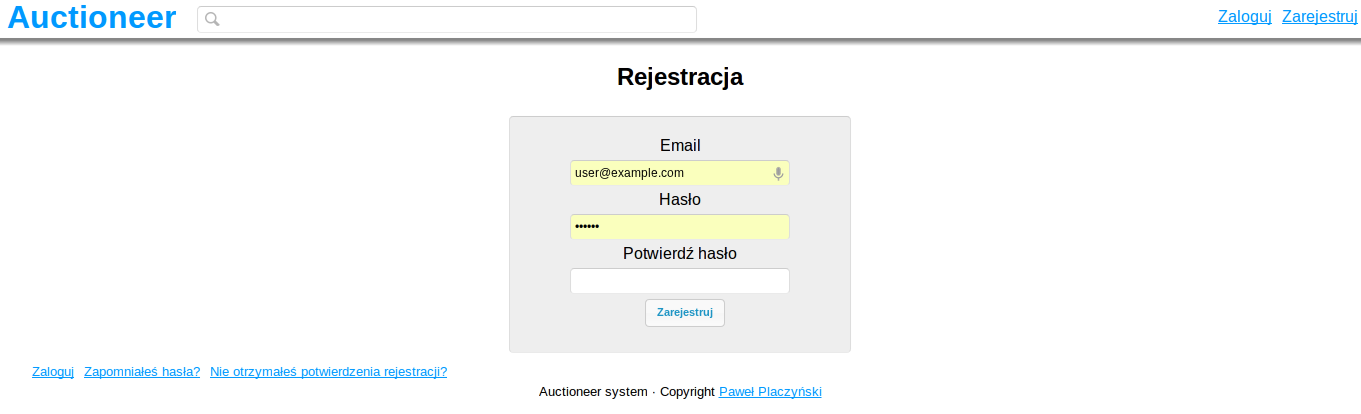
\includegraphics[width=\textwidth]{obrazki/auctioneer13.png}}
\caption{Ekran rejestracji}
\label{screen13}
\end{figure}

Zestaw przycisków: ,,Wstecz'', ,,1'', ,,2'', \ldots, ,,Dalej'' pozwala przeglądać kolejne strony wystawionych aukcji (mechanizm ,,paginacji stron'').


\paragraph{Aukcje}

Na stronie głównej znajduje się lista aukcji. Każda aukcja ma~przy swoim opisie przycisk ,,Więcej'' prowadzący do~strony aukcji (Rys. \ref{screen09} oraz Rys. \ref{screen05}).

\begin{figure}[h]
\centering
\fbox{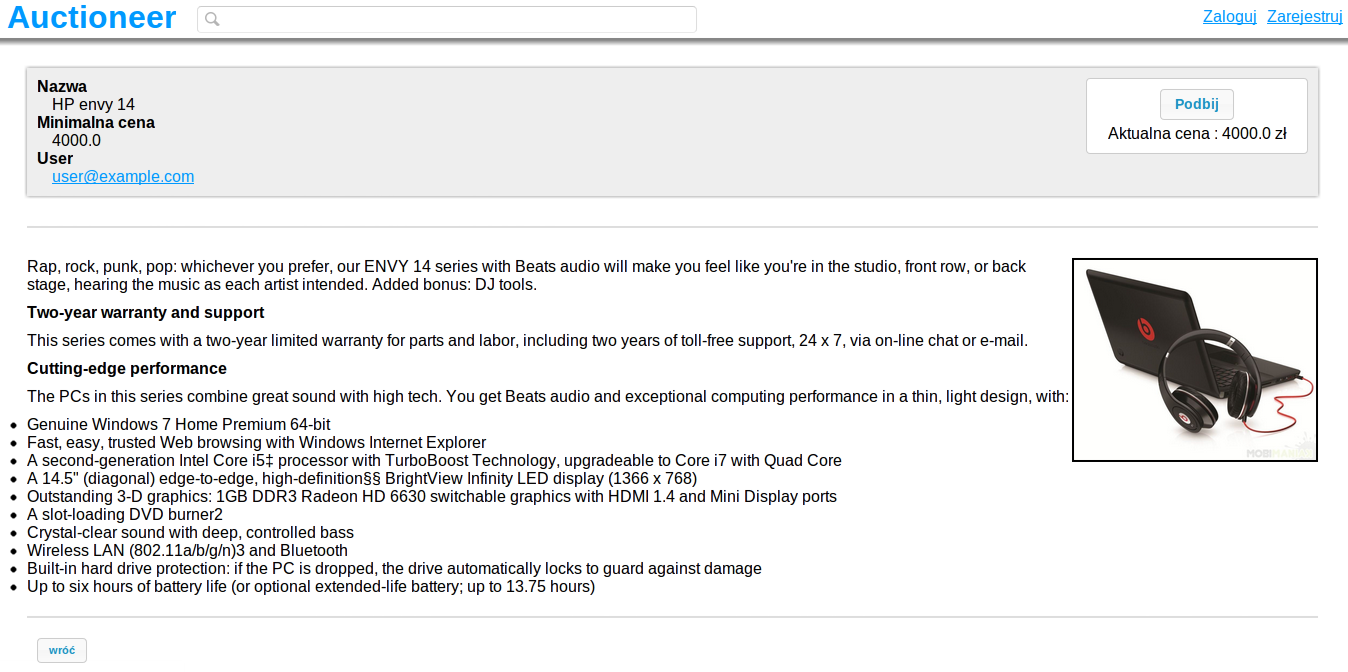
\includegraphics[width=\textwidth]{obrazki/auctioneer09.png}}
\caption{Strona aukcji zawierająca detale. Widok dla gościa lub zalogowanego użytkownika nie wystawiającego aukcję}
\label{screen09}
\end{figure}

\begin{figure}[h]
\centering
\fbox{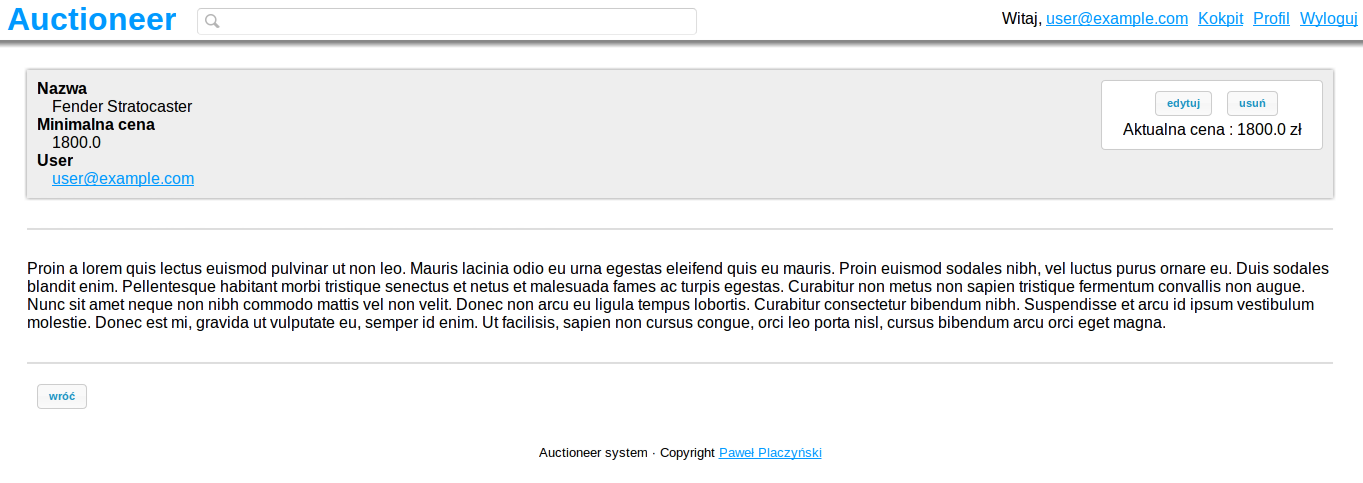
\includegraphics[width=\textwidth]{obrazki/auctioneer05.png}}
\caption{Strona aukcji zawierająca detale. Widok dla zalogowanego użytkownika wystawiającego aukcję}
\label{screen05}
\end{figure}

Strona aukcji zawiera pełny opis wystawionej aukcji. Przycisk ,,Wróć'' pozwala wrócić na~stronę główną, a przycisk ,,Podbij'' prowadzi do~formularza podbijania aukcji (Rys. \ref{screen10}). Jeśli użytkownik nie jest zalogowany to~po~naciśnięciu przycisku ,,Podbij'' zostaje on~przekierowany do~formularza logowania. Po~prawidłowym zalogowaniu, użytkownik zostaje automatycznie przekierowany do~formularza podbijania aukcji.

\begin{figure}[h]
\centering
\fbox{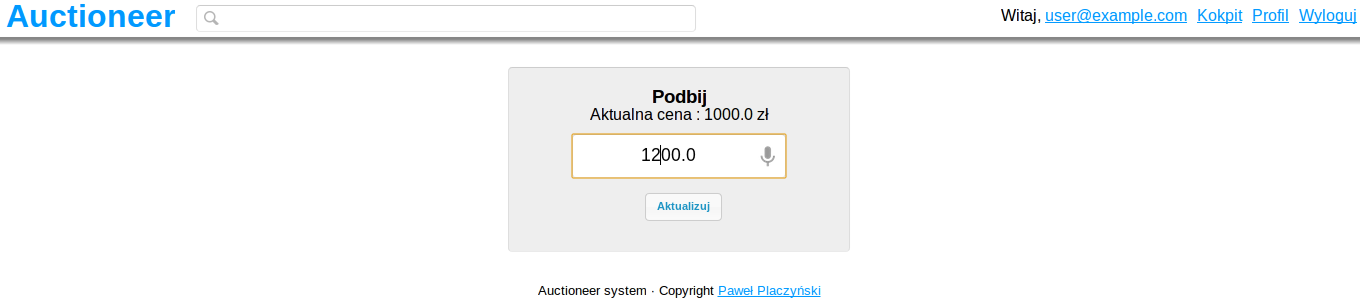
\includegraphics[width=\textwidth]{obrazki/auctioneer10.png}}
\caption{Formularz podbijania aukcji}
\label{screen10}
\end{figure}

\paragraph{Formularz logowania}

Formularz logowania umożliwia niezalogowanemu użytkownikowi otworzyć nową, bezpieczną sesję. Pola tekstowe pozwalają na~wprowadzenie danych logowania: adresu e-mail oraz hasła. Użycie opcji ,,Zapamiętaj mnie'' skutkuje tym, że~sesja użytkownika nie wygaśnie, gdy użytkownik będzie nieaktywny przez dłuższy czas. Przycisk ,,Zaloguj'' służy do~zatwierdzenia operacji logowania.


Jeżeli operacja logowania przeszła pomyślnie (użytkownik o~podanym adresie e-mail oraz haśle posiada konto w~serwisie oraz~zostało aktywowane, ponadto adres e-mail oraz hasło zostały poprawnie podane), to~otwarta zostaje sesja użytkownika oraz zostanie on~przekierowany do~panelu użytkownika. Akcje dla zalogowanego użytkownika opisuje podrozdział \ref{man.user}.

Pod formularzem znajdują się odnośniki pomagające użytkownikowi zarejestrować się, bądź odzyskać utracone hasło. Link ,,Zarejestruj'' przekierowuje do~formularza rejestracji, link ,,Zapomniałeś hasła?'' przekierowuje do~formularza zmiany hasła (Rys. \ref{screen11}), natomiast link ,,Nie otrzymałeś potwierdzenia rejestracji?'' przekierowuje do~formularza ponownego wysłania potwierdzenia rejestracji, gdy takie potwierdzenie nie zostało poprawnie wysłane na~adres e-mail użytkownika (Rys. \ref{screen12}).

\begin{figure}[h]
\centering
\fbox{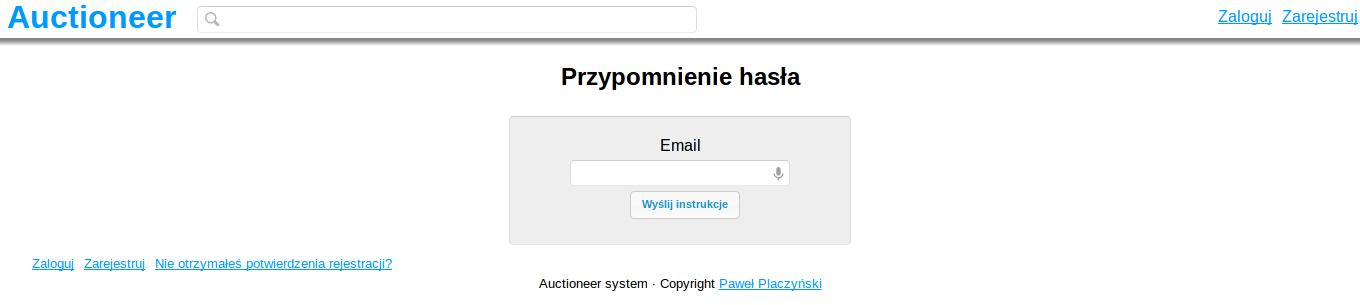
\includegraphics[width=\textwidth]{obrazki/auctioneer11.png}}
\caption{Formularz przypomnienia hasła}
\label{screen11}
\end{figure}

\begin{figure}[h]
\centering
\fbox{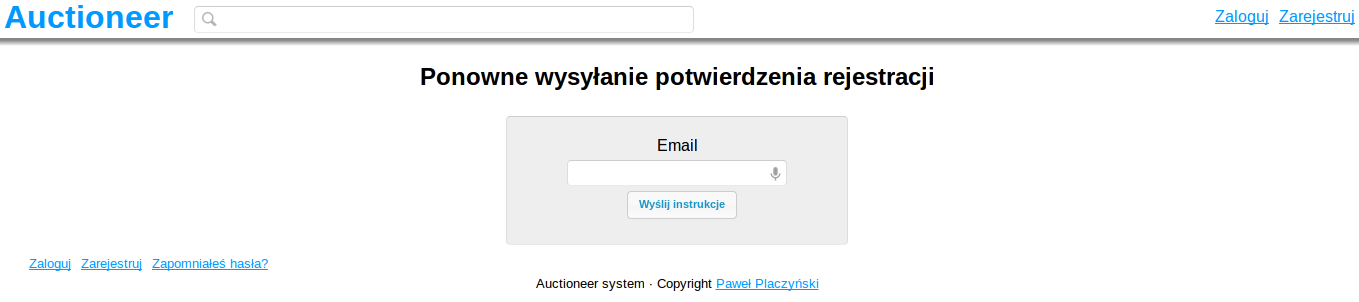
\includegraphics[width=\textwidth]{obrazki/auctioneer12.png}}
\caption{Formularz ponownego wysłania potwierdzenia rejestracji}
\label{screen12}
\end{figure}

\subsection{Opis projektu od~strony użytkownika} \label{man.user}

\paragraph{Panel użytkownika (Kokpit)}

Po~zalogowaniu, użytkownik zostaje przekierowany do~panelu użytkownika (Rys. \ref{screen04}). W~,,nagłówku'' strony znajduje się zestaw odnośników: link ,,Kokpit'' prowadzi do~panelu użytkownika, link ,,Profil'' prowadzi do~formularza edycji profilu (Rys. \ref{screen07}), a~link ,,Wyloguj'' zamyka sesję użytkownika i~przekierowuje na~stronę główną.

\begin{figure}[h]
\centering
\fbox{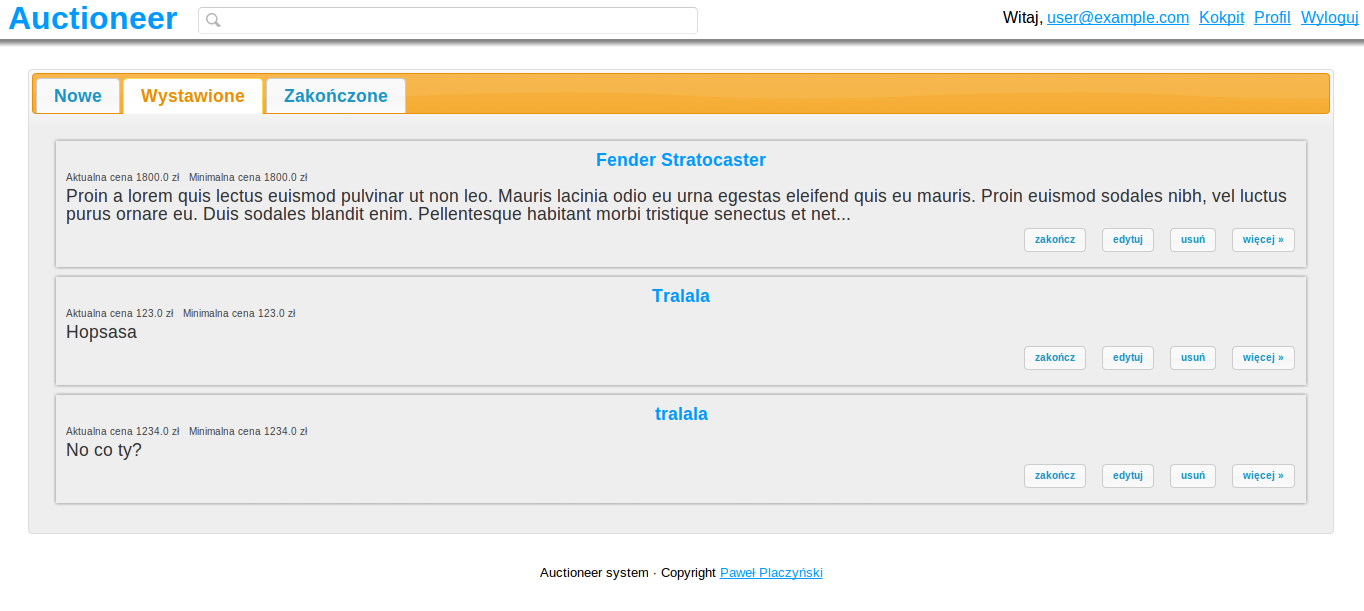
\includegraphics[width=\textwidth]{obrazki/auctioneer04.png}}
\caption{Kokpit użytkownika wraz z~listami aukcji użytkownika}
\label{screen04}
\end{figure}

\begin{figure}[h]
\centering
\fbox{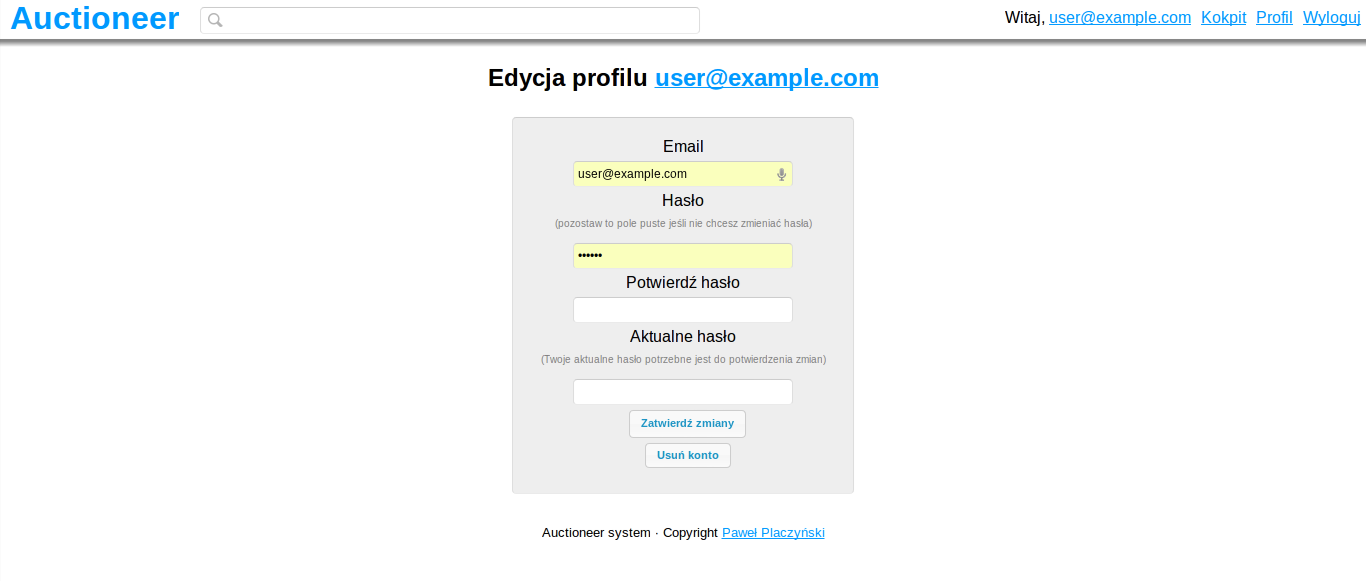
\includegraphics[width=\textwidth]{obrazki/auctioneer07.png}}
\caption{Panel edycji profilu użytkownika}
\label{screen07}
\end{figure}

Na~panelu użytkownika widoczne są zakładki: \textit{Nowe}, \textit{Wystawione}, \textit{Zakończone}, \textit{Wygrane}. Otwierają one kolejno: listę nowo utworzonych aukcji użytkownika, listę aukcji aktualnie wystawionych przez użytkownika, listę aukcji zakończonych oraz listę aukcji wygranych przez użytkownika.


Każda aukcja, z~dowolnej, wyżej wymienionej listy, posiada dwa przyciski: ,,edytuj'' -- prowadzący do~formularza edycji aukcji (Rys. \ref{screen06}) oraz ,,usuń'' -- powodujący usunięcie aukcji po~uprzednim potwierdzeniu operacji. Ponadto aukcja posiada przyciski zmiany stanu: aukcje z~listy \textit{Nowe} posiadają przycisk ,,wystaw'', aukcje z~listy \textit{Wystawione} -- ,,zakończ'' oraz~aukcje z~listy \textit{Zakończone} -- ,,wystaw ponownie''.

\begin{figure}[h]
\centering
\fbox{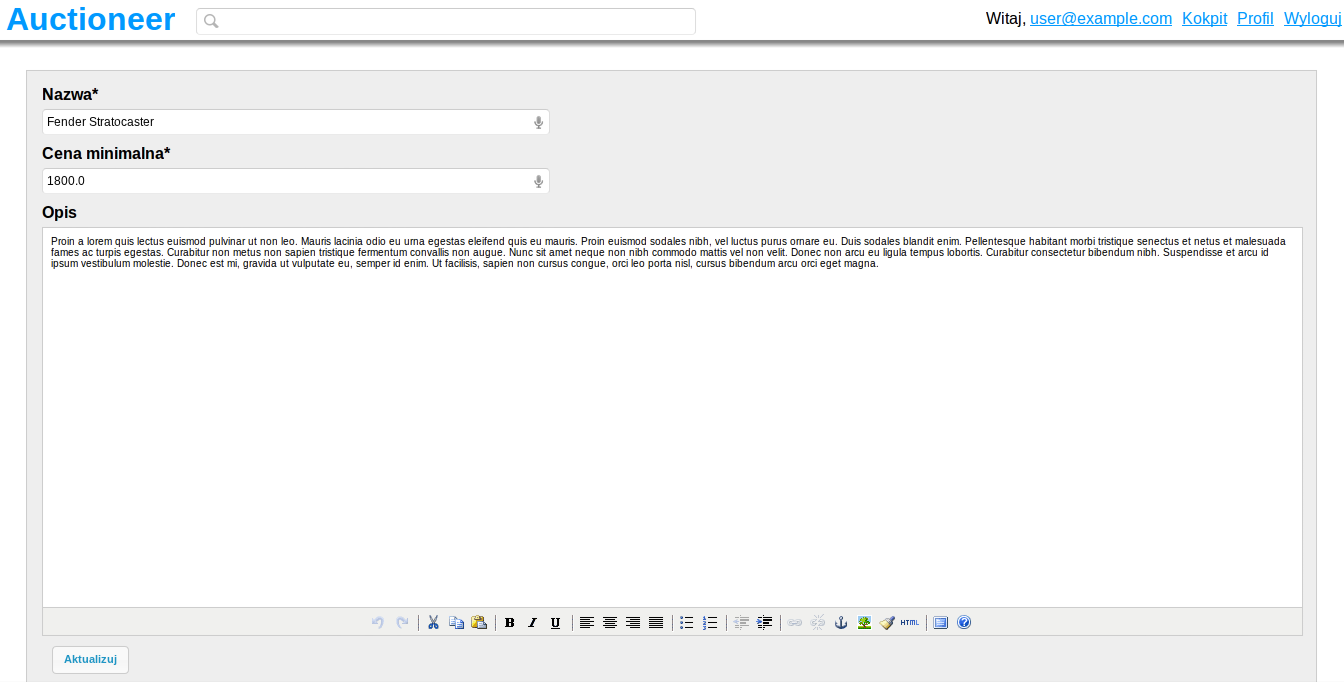
\includegraphics[width=\textwidth]{obrazki/auctioneer06.png}}
\caption{Panel edycji aukcji}
\label{screen06}
\end{figure}

\paragraph{Panel edycji aukcji}

Panel edycji aukcji posiada pole tekstowe zmiany nazwy (tytułu) aukcji, pole tekstowe zmiany ceny minimalnej aukcji oraz pole tekstowe zaopatrzone w~zestaw narzędzi, służących do~formatowania tekstu, do~edycji opisu aukcji. Przycisk ,,Aktualizuj'' zatwierdza zmiany.

\subsection{Opis projektu od strony administratora}

Aby odwiedzić panel administratora (Rys. \ref{screen08}) należy podać ścieżkę \textit{adres\_bazowy\_aplikacji}\texttt{/admin}. Wyświetli się wówczas formularz logowania administratora. Podając odpowiednie dane (adres e-mail oraz hasło) można zarządzać aplikacją z~poziomu administratora.

\begin{figure}[h]
\centering
\fbox{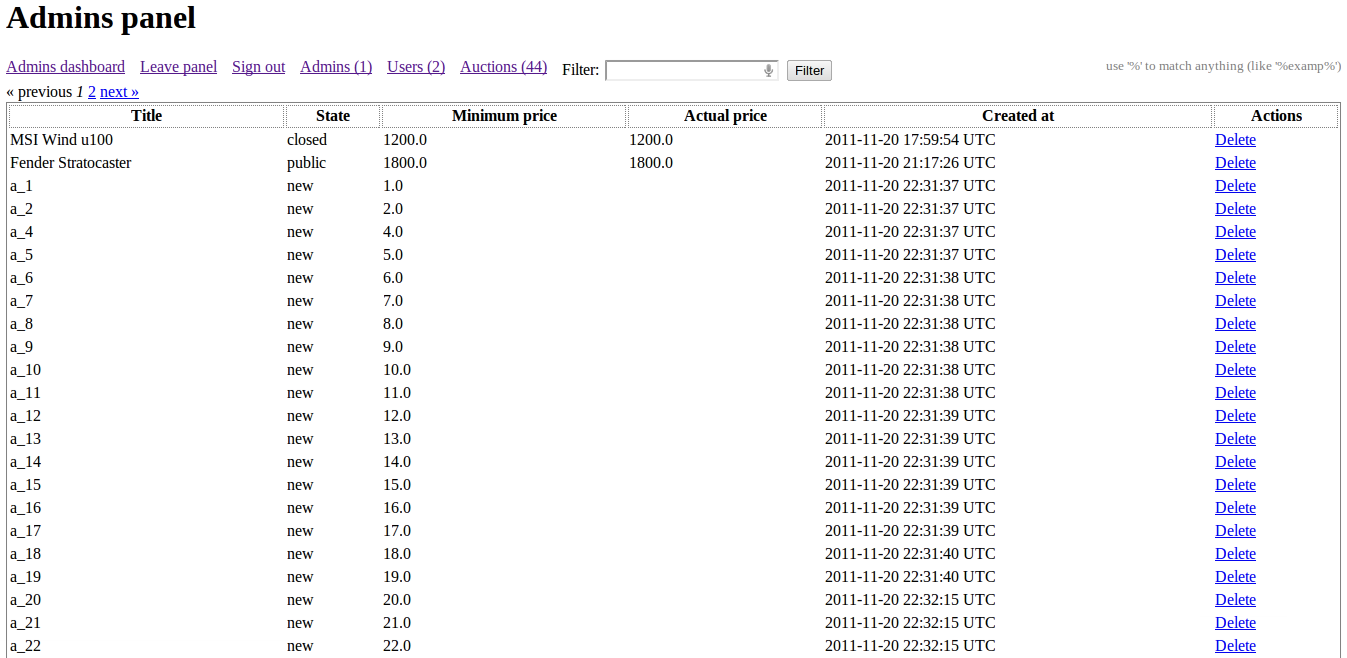
\includegraphics[width=\textwidth]{obrazki/auctioneer08.png}}
\caption{Panel administratora z~listą aukcji}
\label{screen08}
\end{figure}

W~panelu administratora znajdują się:

\begin{itemize}
  \item Link ,,Leave panel'', który pozwala wyjść z~panelu, pozostając zalogowanym jako administrator. Link ten przekierowuje na~stronę główną.
  \item Link ,,Sign out'' umożliwia wylogowanie administratora.
  \item Link ,,Admins'' pokazuje listę administratorów serwisu. Lista ta~udostępnia następujące akcje: wyszukanie administratora według adresu e-mail (pole tekstowe oznaczone etykietą ,,Filter'') oraz usunięcie administratora (link ,,Delete'', przy czym nie jest możliwe usunięcie aktualnie zalogowanego administratora).
  \item Link ,,Users'' pokazuje listę użytkowników. Lista ta~pozwala na~wyszukanie użytkownika według adresu e-mail (pole tekstowe oznaczone etykietą ,,Filter''), usunięcie użytkownika (link ,,Delete'') oraz zalogowanie się jako użytkownik (link ,,Login'').
  \item Link ,,Auctions'' pokazuje listę aukcji. Lista pozwala na~wyszukanie aukcji według tytułu lub opisu aukcji (pole tekstowe ,,Filter'') oraz usunięcie aukcji (link ,,Delete'').
\end{itemize}
